% !TeX spellcheck = en_US
\chapter{Introduction}
%one paragraph per item of the abstract. However, provide more details and do not just copy sentences from the abstract. 
%Additionally, provide  another paragraph and  Make your own \textbf{contribution(s)} explicit ("The contribution of this thesis is...").

% Context / Motivation
In the dynamic field of smart home technologies, users are increasingly turning to sophisticated automation systems to optimize their everyday lives.
As the complexity of these systems continues to grow \cite{technologies11010009}, there arises a pressing need for innovative solutions that empower users with a deeper understanding of their environments \cite{baby_home_2017}. 
Picture a user with a huge amount of automations in their smart home, occupyied with complex questions like, ``Why did I have higher heating costs this winter?'' or ``What was the intention behind the light just turning on in the kitchen?''
While technology-interested users may attempt to answer such questions themselves through self-analysis of their smart home systems, the complexity of such tasks can be time-consuming and may not be simply feasible for everyone.
These scenarios encapsulate the motivation behind this thesis, which centers on the development of a chatbot for smart home systems and home automation.
The primary focus is increasing system explainability and addressing the unique challenges users encounter in analyzing the intricacies of their smart homes.

Furthermore, the implementation of a chatbot functionality holds the potential for additional benefits, including a reduction in support requests as users gain autonomy in troubleshooting \cite{HUANG2024103600} which is also available at any time. 
By storing and analyzing user requests, the system could also provide insights into the needs and interests of users and thus influence future developments. 
Moreover, the chatbot could act as a valuable tool in identifying unintended behavior or bugs within the smart home system, contributing to a more robust and user-friendly technology landscape.

% Problem
%-users are confronted with a lack of tools that can effectively provide insights into the rationale behind system actions
%-inconsistencies in the "decisions" of smart home devices --> user and developers want to understand
%-absence of a reference architecture for a chatbot tailored to answer complex questions in a smart home environment
When it comes to smart home technology, users face a variety of difficulties that draw attention to important issues that call for creative solutions. First and foremost, users are confronted with a lack of tools capable of effectively providing insights into the rationale behind system actions \cite{kok2022explainableartificialintelligencexai}.
Even when we look at less complex use cases like managing smart home devices there is for example no good solution to get an overview of the device one has or basic analysis like ``Is any window open?''.
Inconsistencies in the ``decisions'' of smart home devices extend the problems even further, as developers and users can struggle to comprehend the underlying logic of actions that are executed \cite{kok2022explainableartificialintelligencexai}, with the added challenge of distinguishing whether the observed behavior is indicative of a potential bug or a result of a specific user configuration.

A hurdle for the planned development throughout this thesis is the lack of a reference architecture designed especially for chatbots to answer complicated queries inside a smart home system.
Therefore it has to be analyzed if there exist related work on chatbots which answer complex questions in a similar way to potentially inspire this work.

Another problem for the thesis is the lack of available data in the Bosch Smart Home system in which the chatbot should be integrated.
This deficiency manifests in several dimensions, beginning with the cost-intensive nature of cloud services and the consequential limitations imposed by a surge in user requests that could occur in requests to a chatbot. 
Compounding this issue, smart home devices have constrained computing resources due to their compact size which may make the accumulation of data about the system difficult or slow. 
The integral role of a knowledge base for chatbot functionality is the center of these problems, as it heavily relies on data. 
In the current state of the Bosch Smart Home System, although valuable data concerning device resources and system logs exists, accessibility remains restricted since logs only get available when users send a support request.
The data of individual smart homes would represent an excellent source for chatbot functionality, including resource metrics such as CPU and RAM usage and logs detailing system actions.
However, the challenges persist, requiring careful consideration of data availability, structuring, and integration into the chatbot's architecture to form a reliable knowledge base. 
These data-related challenges come together to the pressing need for innovative solutions to enhance the data accessibility and usability of smart home systems \cite{7753232}.

%    - cost-intensity through cloud services and huge amount of requests 
%   - limited ressources due to device size
%    - A knowledge base is a crucial part of chatbots which is based on data--
%    - state in Bosch Smart Home System is that data about devices is available but not accessable without a request to the user support.
%        --> this data consists of ressource data (cpu usage, ram usage, ...) and logs (containing system actions like turning devices on or off)
%    - depending on the architecture of the chatbot the data has to be available and possibly be structured to form a reliable knowledge base


% Objective
The objectives of this thesis are multifaceted, aiming to find important aspects in developing a functional chatbot tailored for answering complex questions and managing devices in the area of smart homes. The first goal is to understand the key components needed to create a functioning chatbot. This involves identifying requirements and evaluating tools suitable for building a chatbot, with a specific focus on the feasibility of utilizing open-source options to answer if they effectively can contribute to such a project.

Subsequently, the research attempts to push the boundaries of chatbot capabilities by exemplarily developing a chatbot into the Bosch Smart Home app and testing how far such a system can go in answering complex questions. The general question here is whether it is even plausible to develop a chatbot for the mentioned application. This objective involves finding and assessing the technical limitations and potential breakthroughs in creating an adaptable chatbot for this specific domain.

Finally, by providing explainability for users, the thesis seeks to satisfy the user-centric aspect of smart home technologies. This objective involves developing features within the chatbot that not only answer questions but also offer transparent and understandable explanations regarding the actions and decisions made by the smart home system. This user-focused approach seeks to enhance the overall user experience and potentially bring benefits as comprehension and trust to users about their own smart home. 

%  Method:
\begin{figure}[b]
\centering
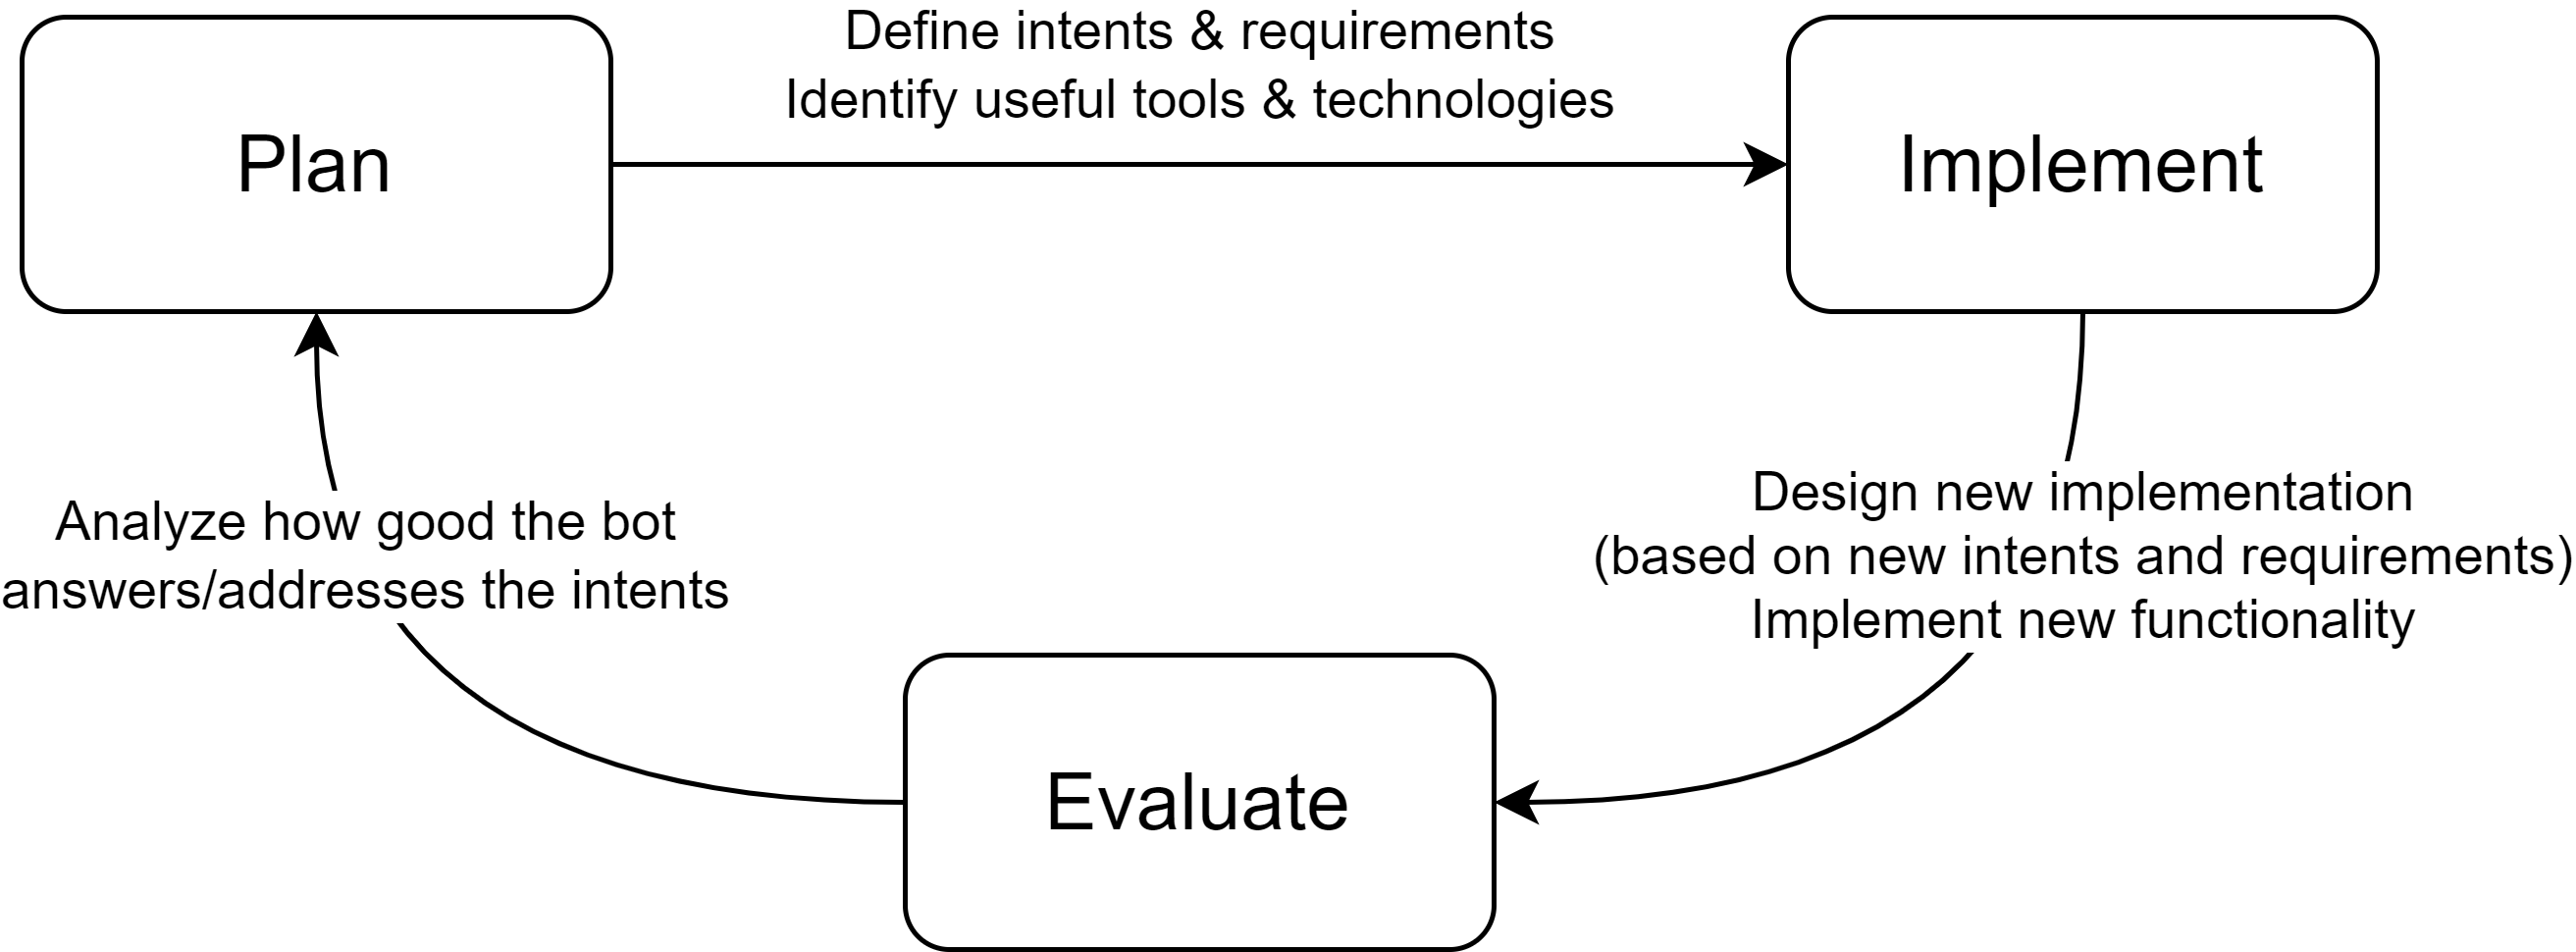
\includegraphics[width=0.8\textwidth]{graphics/iterative-design.png}
\caption{Visualization of the Iterative Development Process}
\label{fig:iterative-design}
\end{figure}
The research methodology for this thesis involves an iterative development process, which is shown in \cref{fig:iterative-design}. This approach includes defining intents and requirements, selecting tools and technologies, implementing a chatbot prototype, and conducting a thorough evaluation. Detailed information on the methodology can be found in \cref{chap:method}.

% todo Result
The thesis employs a strict evaluation methodology, combining quantitative metrics for model performance with qualitative user studies to assess the chatbot's impact on system explainability and user satisfaction.
The  findings indicate that the implemented chatbot enhances the usability and explainability of smart home systems within the Bosch Smart Home environment. Evaluation metrics combining semantic similarity and JSON accuracy demonstrate the chatbot's capability to handle diverse intents such as device control and data analysis tasks effectively. One of our customized models (``shllama3instruct'') emerged as the top performer, achieving a balanced approach between helpful answers and precise \gls{json} function execution to control devices.
However, participants of our study expressed uncertainty about preferring the chatbot over traditional interfaces. Additionally, challenges remain, such as the chatbot not always responding in the same language used by the user.

% Contributions [explicit]
\section{Explicit Contributions}
This thesis advances smart home automation by developing a user-friendly, explainability-enhancing chatbot and providing a practical architecture for integrating large language models into smart home environments without extensive fine-tuning. 
It offers novel insights into chatbot architectures, tools, and methodologies for answering complex questions within smart home systems, particularly the Bosch Smart Home environment. 
While integrating a chatbot into smart homes proves challenging for complex intents, it presents unique opportunities for providing insights otherwise unattainable. 
The research assesses the chatbot's capabilities, addresses potential implementation challenges, and offers recommendations for future developments. 
Ultimately, this work aims to deepen users' understanding of their smart homes, enhancing transparency and usability of home automation systems, contributing valuable knowledge to both academic and industry spheres in the rapidly evolving field of smart home technologies.

\section{Cooperation with Bosch Smart Home}
This thesis is conducted in collaboration with Bosch Smart Home, a leader in home automation technology. Bosch Smart Home, part of the Bosch Group, specializes in innovative solutions to enhance comfort, security, and energy efficiency.
Our partnership focuses on exploring the integration of a chatbot into the Bosch Smart Home system. This cooperation ensures that the research findings are practically relevant and directly applicable and also provides a smart home system to build the chatbot on.

\newpage
\section*{Thesis Structure}
The structure of this thesis is the following:
\begin{description}
    \item[Chapter~\ref{chap:foundation} -- \nameref{chap:foundation}] This chapter lays the groundwork by discussing foundational concepts and reviewing related work in the field of smart home chatbots.
    \item[Chapter~\ref{chap:method} -- \nameref{chap:method}] This chapter outlines the methodology, detailing the iterative process used for developing and refining the chatbot, including expert interviews and user surveys.
    \item[Chapter~\ref{chap:concept} -- \nameref{chap:concept}] This chapter presents the concept for the chatbot, including the definition of intents, architecture design, and requirements gathered from preliminary research.
    \item[Chapter~\ref{chap:implementation} -- \nameref{chap:implementation}] This chapter details the implementation of the chatbot, discussing the technology stack, server and client components, interaction flow, and challenges encountered during development.
    \item[Chapter~\ref{chap:evaluation} -- \nameref{chap:evaluation}] This chapter provides a comprehensive evaluation of the chatbot's performance. It includes the study design, performance metrics, user experience feedback, results of the evaluation, a discussion of the findings, and an analysis of potential threats to validity.
    \item[Chapter~\ref{chap:conclusion} -- \nameref{chap:conclusion}] This chapter concludes the thesis, summarizing findings, discussing the implications, suggesting directions for future research, and reflecting on the limitations and lessons learned.
\end{description}
